Pulsars can be observed by measuring the variation in amplitude of the radio
waves from a particular sky location. A single observation consists of measuring
the amplitude over a period of approximately $30$ minutes or so, which for pulsars
with periods $\sim 1$~s, means recording up to several thousand individual pulsations.

The shape of individual pulses can vary substantially during a single
observation; to show this, in Fig.~\ref{fig: CP1919 stacked}, successive pulses
from the first pulsar discovered, PSR B1919+21, are vertically stacked and
aligned illustrating typical variations.
\begin{figure}[htb]
\centering
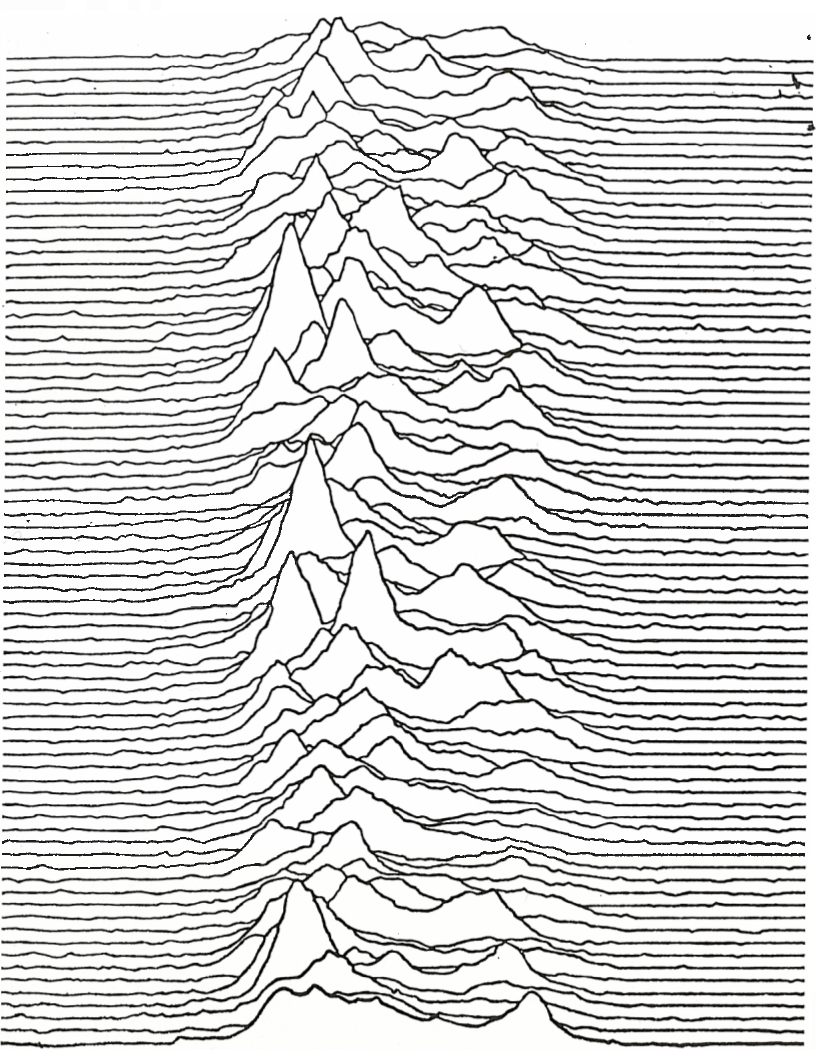
\includegraphics[width=0.5\textwidth]{CP1919_stacked}
\caption{The radio amplitude of successive pulses from PSR~B1919+21 stacked
vertically, figure reproduced from \citet{mitton1977cambridge}, originally
produced by \citet{craft1970}.}
\label{fig: CP1919 stacked}
\end{figure}
Each pulsation lasts for a small fraction of the pulse period. As an example,
the pulses in PSR~B1919+21, shown in Fig.~\ref{fig: CP1919 stacked}, have
typical widths of $0.031$~s, but the pulse period is $1.337$~s; note that the
stacked plot truncates each pulsation to show only the pulsation itself. Later
on in Fig.~\ref{fig: pop stats others} we will show this to be true for the
normal radio pulsar population by looking at the duty-cycle, the ratio of the
pulse duration to the pulse period.

In order to understand the gross features of a pulsar, astronomers average over
the hundreds to thousands of pulses observed during a single observation to
create a single integrated pulse profile. This is done by sampling the radio
signal at fixed time intervals then `folding' all the samples at the pulse
period (for a complete review see \citet{Lyne2012book}). The integrated pulse
profile of a pulsar looks similar to any of the individual pulses seen in
Fig.~\ref{fig: CP1919 stacked}, but in contrast to the individual pulses which
create it, it can be highly stable when measured independently over timescales
of years.

The integrated pulse profile not only gives a stable picture of what the
pulsations look like on average, but it also provides a highly accurate
measurement of the time of arrival (TOA) of a single pulse during the
observation; which pulse depends on how the folding is done. It is this TOA
which can be used to `time' a pulsar. To do this, regular observations of a
pulsar must be made every few months or so, each observation results in a
precise TOA measurement. Having obtained a series of TOAs, pulsar astronomers
generate a \emph{timing model} which attempts to exactly count each and every
pulse. Between any two observations there may be several million pulses so the
timing model needs to account for any mechanisms which may produce variations
in the TOAs.  The process is standardised by the software package
\texttt{TEMPO2} developed by \citet{Hobbs2006}, we will now describe the
essential features.

The TOA of a pulse at the detector on Earth depends on many factors such as the
time at which the beam was directed by source towards the Earth, the relative
motions of the source and detector, and any mechanisms effecting the signal during
its transit. The time at which pulses are generated (when the source beams towards
the earth) are governed by the \emph{timing properties} of the star itself.
As described by \citet{Edwards2006} these can be modelled by a Taylor expansion
in the phase at time $t$ given by
\begin{equation}
\phi(t) = \sum_{n\ge 1}\frac{\nu^{(n-1)}}{n!}(t - \tref)^{n} + \phi_{0}.
\label{eqn: Taylor compact}
\end{equation} 
where $\{\nu^{(n)}\}$ is the frequency $\nu$, spin-down rate $\dot{\nu}$, etc.
of the rotating body, $\phi_0$ is the initial phase, and $\tref$ is an
arbitrary reference time. This expansion is usually truncated at $n=3$, the
second order spin-down rate $\ddot{\nu}$. The timing model then includes
corrections to this to model the relative motion of the source and detector,
intergalactic transit, and other effects; these are described in full in
\citet{Edwards2006}. 

Between any two TOAs, if the timing model is correct, an integer number of
rotations must have occurred; this allows the use of the deviation of
$\phi(t_{TOA}^{j})$ from an integer as a test statistic. The timing model
minimises the RMS of these deviations with respect to the timing model
parameters, for example the frequency and frequency derivatives. The output of
applying a particular timing model (choice of corrections) and a set of data is
then the best-fit of these parameters and an estimate of their associated
errors.  The corrections applied in a timing model provide a method to
investigate pulsar physics: for example in some pulsar an orbital correction
must be applied which models the periodic motion of the star due to an orbital
companion. Using this technique, \citet{wolszczan1992planetary} discovered the
first \emph{exoplanet} orbiting the pulsar PSR~B1257+12.

A minimisation of the timing model parameters will converge regardless of
whether of not the model itself is appropriate. To qualitatively check if the
fitted model described the data, pulsar astronomers refer to the \emph{timing
residual}, which is the difference between the TOA, as given by the timing
model, and the actual TOA. The timing residual provides a mechanism to evaluate
the timing model: a periodic variation in the timing residual with period
$365$~days, may indicate the correction of the Earth's orbit about the Sun may
be incorrect. If the timing model is correct, the residual data points should
be gaussianly distributed around zero. A timing model is described as
\emph{phase-connected} if it is accurate enough to track the pulsar to within a
single rotationa.  For most pulsars this is the case and a single set of
coefficients can track the spin-down over periods greater than a year.

However, for many pulsars the timing residual contains `structure' known as
\emph{timing variations} which cannot be associated with any known correction.
These variations are the focus of this work and we will describe the details
further in Sec.~\ref{sec: timing variations}.  In the next section, we will
describe the variety of known pulsars which have been timed using this method.


